\documentclass[tikz,border=9pt]{standalone}
\usepackage{amsmath,amssymb}
\usetikzlibrary{arrows.meta,positioning,calc}
\begin{document}
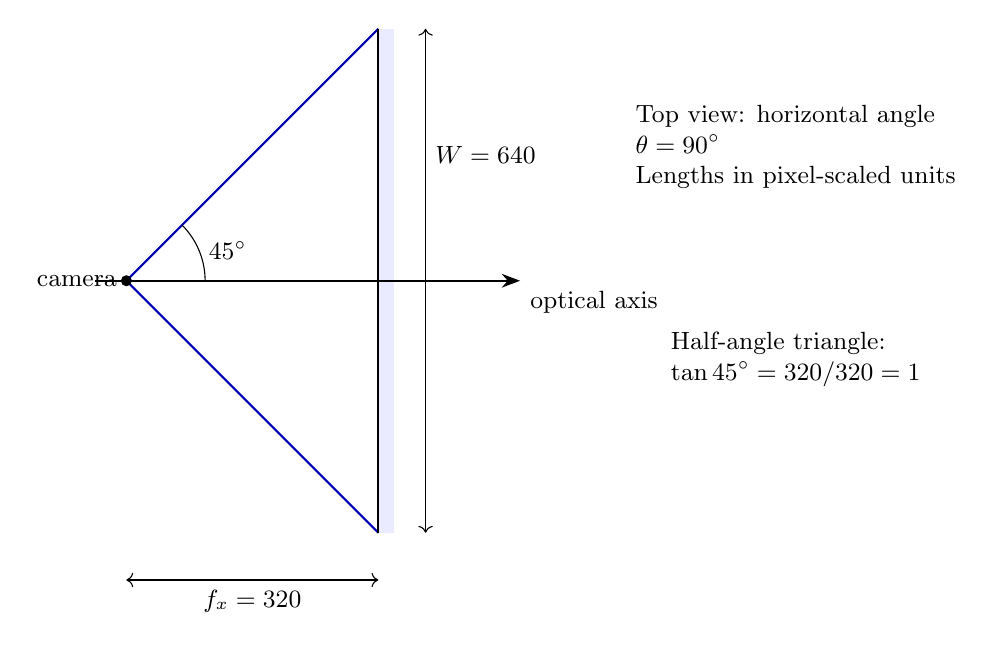
\begin{tikzpicture}[font=\small,arr/.style={-{Stealth},thick},box/.style={draw=blue!55!black,rounded corners,fill=blue!4,align=center,text width=2.9cm,minimum height=1.05cm}]

\coordinate (C) at (0,0);
\fill[blue!8] (3.2,-3.2) rectangle (3.4,3.2);
\draw[arr] (-.4,0)--(5,0) node[below right]{optical axis};
\draw[thick,blue!70!black] (C)--(3.2,3.2) (C)--(3.2,-3.2);
\draw[thick] (3.2,-3.2)--(3.2,3.2);
\draw[<->] (3.8,-3.2)--(3.8,3.2) node[pos=.75,right]{$W=640$};
\draw[<->] (0,-3.8)--(3.2,-3.8) node[midway,below]{$f_x=320$};
\draw (1,0) arc(0:45:1) node[midway,right]{$45^\circ$};
\fill (C) circle(2pt) node[left]{camera};
\node[align=left] at (8.5,1.7){Top view: horizontal angle\\$\theta=90^\circ$\\Lengths in pixel-scaled units};
\node[align=left] at (8.5,-1){Half-angle triangle:\\$\tan45^\circ=320/320=1$};

\end{tikzpicture}
\end{document}
